\documentclass[12pt]{article}
\usepackage[a4paper, margin=1in]{geometry} 
\usepackage{graphicx} 
\usepackage{hyperref}
\usepackage{float}
\usepackage{multicol}
\usepackage{multirow}
\usepackage{amsmath}
\usepackage[ruled]{algorithm2e}
\usepackage{amssymb}
\usepackage[font=small, labelfont=bf]{caption}
\usepackage[table,xcdraw]{xcolor}

\title{Lecture Notes for \\ INF281 Basics of Bioinformatics Sequence Analysis}
\author{Takaya Saito}
\date{}

\begin{document}

\pagenumbering{arabic}
\setcounter{page}{54}

\makeatletter 
\renewcommand{\thefigure}{\arabic{section}.\arabic{figure}}
\renewcommand{\thetable}{\arabic{section}.\arabic{table}}
\makeatother

%
% Model evaluation
%
\setcounter{section}{6}
\setcounter{figure}{0}
\setcounter{table}{0}
\section{Model evaluation}
%\documentclass[12pt]{article}
%\usepackage[a4paper, margin=1in]{geometry} 
%\usepackage{graphicx} 
%\usepackage{hyperref}
%\usepackage{float}
%\usepackage{multicol}
%\usepackage{multirow}
%\usepackage[font=small, labelfont=bf]{caption}
%
%\begin{document}

%
% Evaluation of binary classifiers 
%
\subsection{Evaluation of binary classifiers}
Binary classifiers are mathematical or computational models that classify an input data set and produce the output with two labels. 

%
% Evaluation of models
%
\subsubsection*{Evaluation of models}
The performance of different models can be evaluated under the same test dataset.
\begin{itemize}
\item Algorithms
\item Scoring schemes
\item Statistical analysis
\end{itemize}

%
% Test data
%
\subsubsection*{Test data}
It should contain both homologous and non-homologous alignments.
\begin{itemize}
\item Positive: homologous
\item Negative: non-homologous
\end{itemize}

\begin{figure}[H]
  \centering
      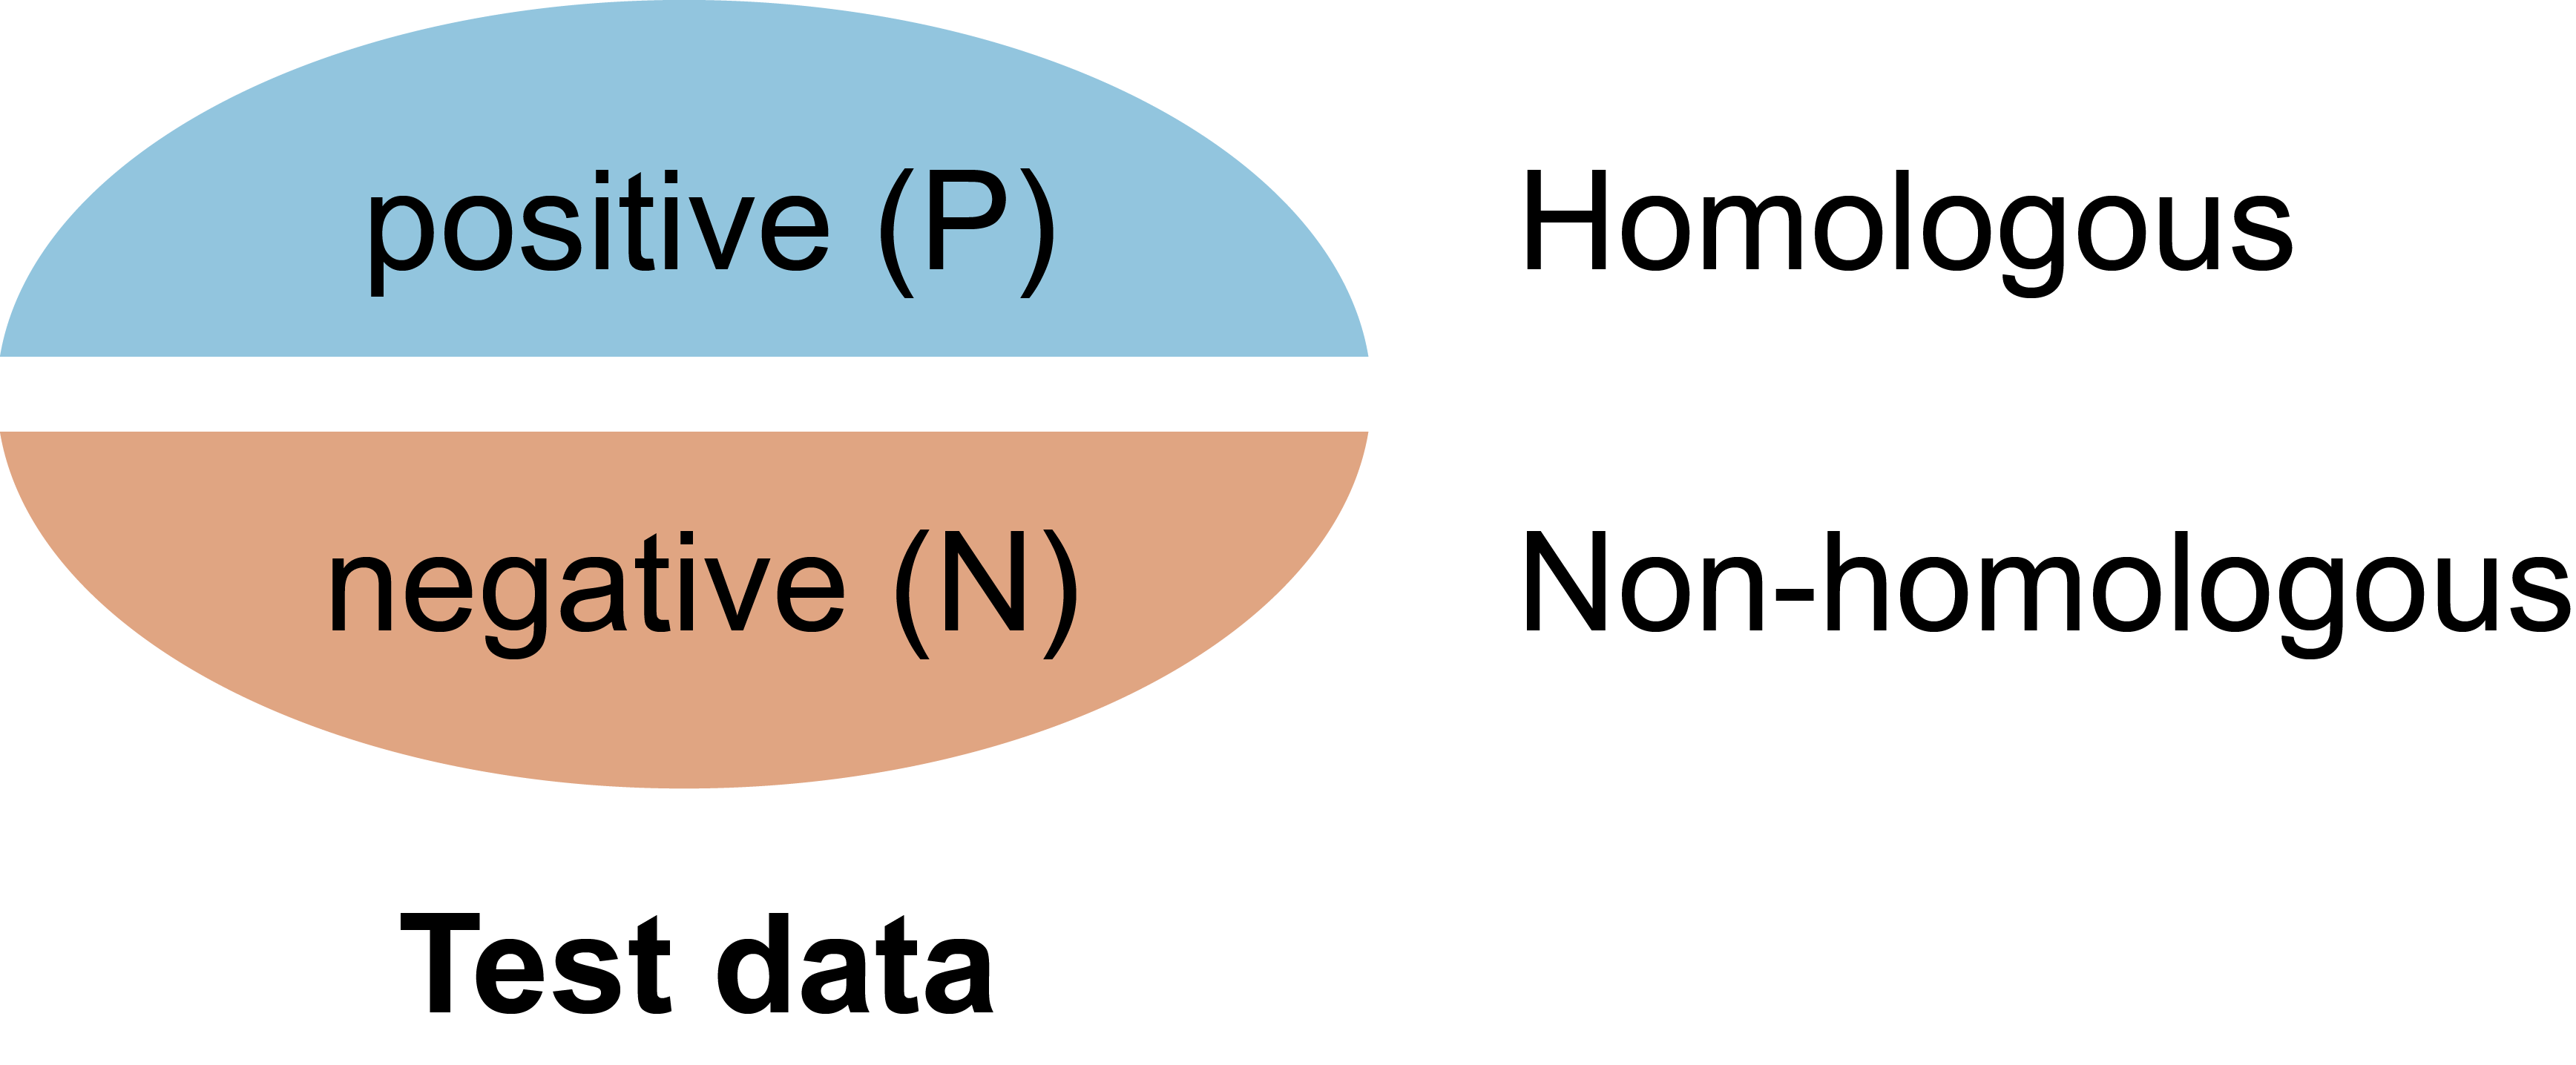
\includegraphics[width=0.4 \textwidth]{fig07/test_data.png}
  \caption{Test dataset for homologous and non-homologous}
\end{figure}

%
% Model output
%
\subsubsection*{Model output} 
Different models often output different formats of scores. 

\begin{itemize}
\item Raw scores, bit scores, z-scores
\item P-values, e-values
\end{itemize}

\noindent
Threshold values are used to separate the result into positives and negatives.

\begin{figure}[H]
  \centering
      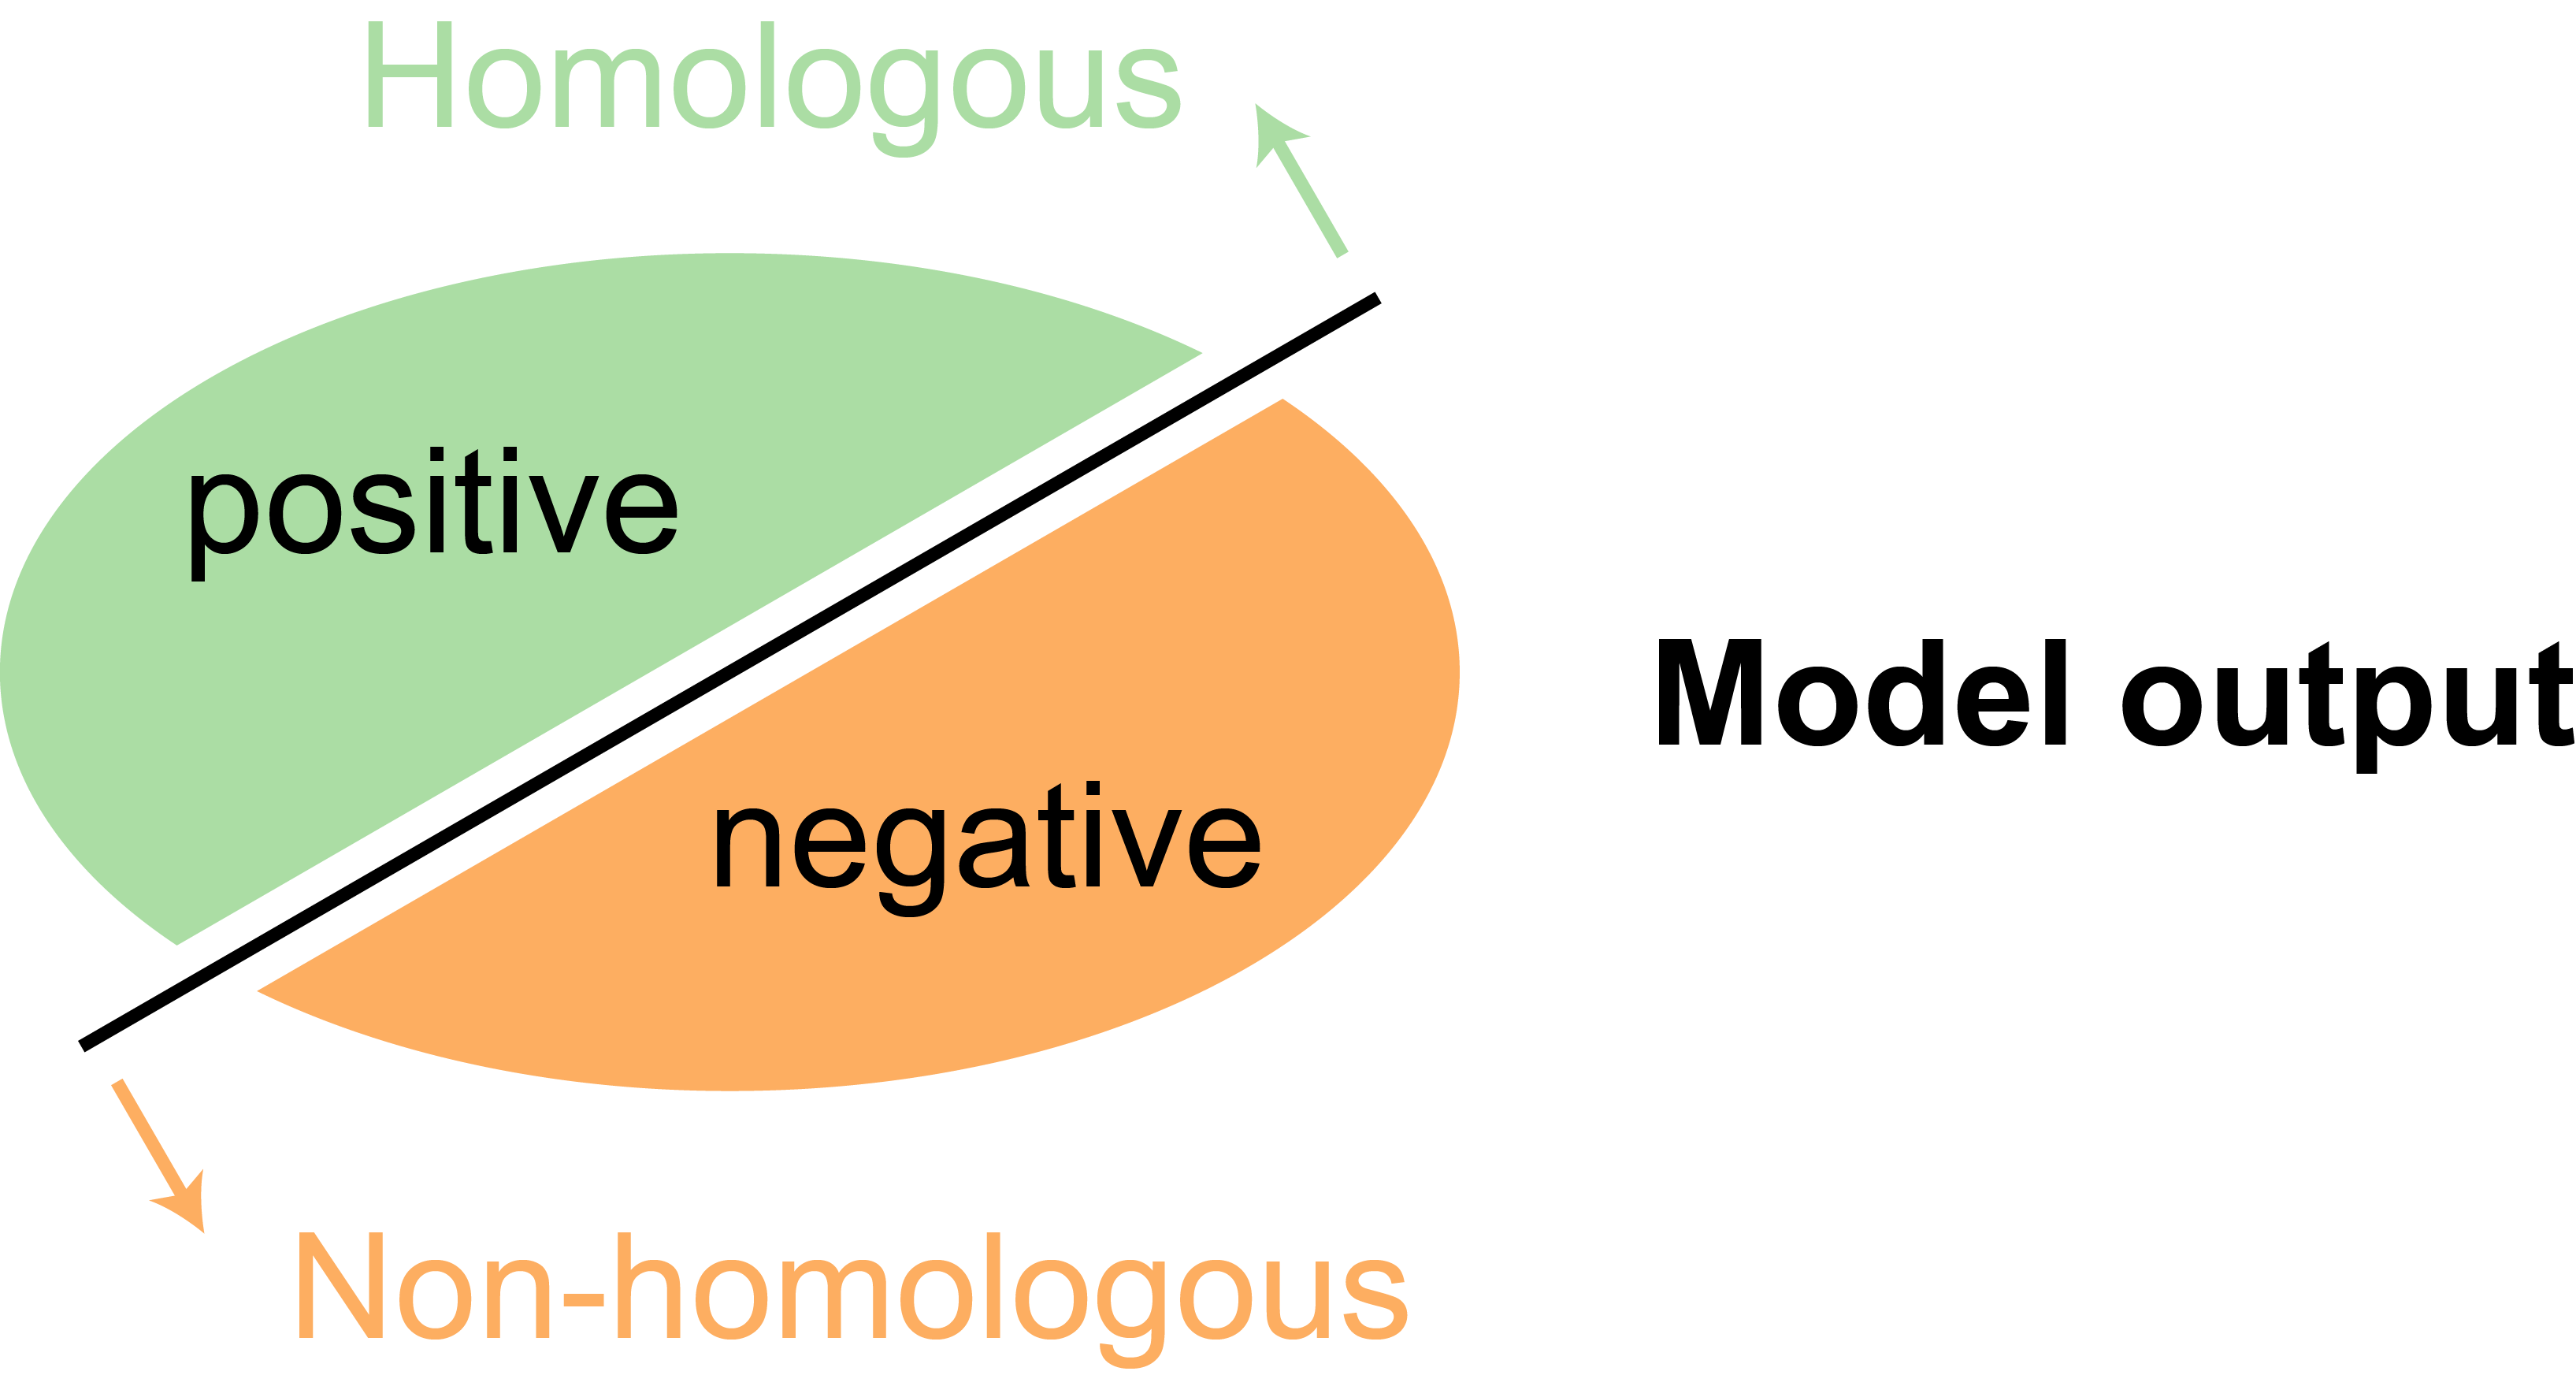
\includegraphics[width=0.4 \textwidth]{fig07/model_output.png}
  \caption{Model output for homologous and non-homologous}
\end{figure}

\bigskip 

%\end{document}

%\documentclass[12pt]{article}
%\usepackage[a4paper, margin=1in]{geometry} 
%\usepackage{graphicx} 
%\usepackage{hyperref}
%\usepackage{float}
%\usepackage{multicol}
%\usepackage{multirow}
%\usepackage[font=small, labelfont=bf]{caption}
%
%\begin{document}

%
% Confusion matrix 
%
\subsection{Confusion matrix}
The output of a model produces two false and two correct classifications. 

\begin{figure}[H]
  \centering
      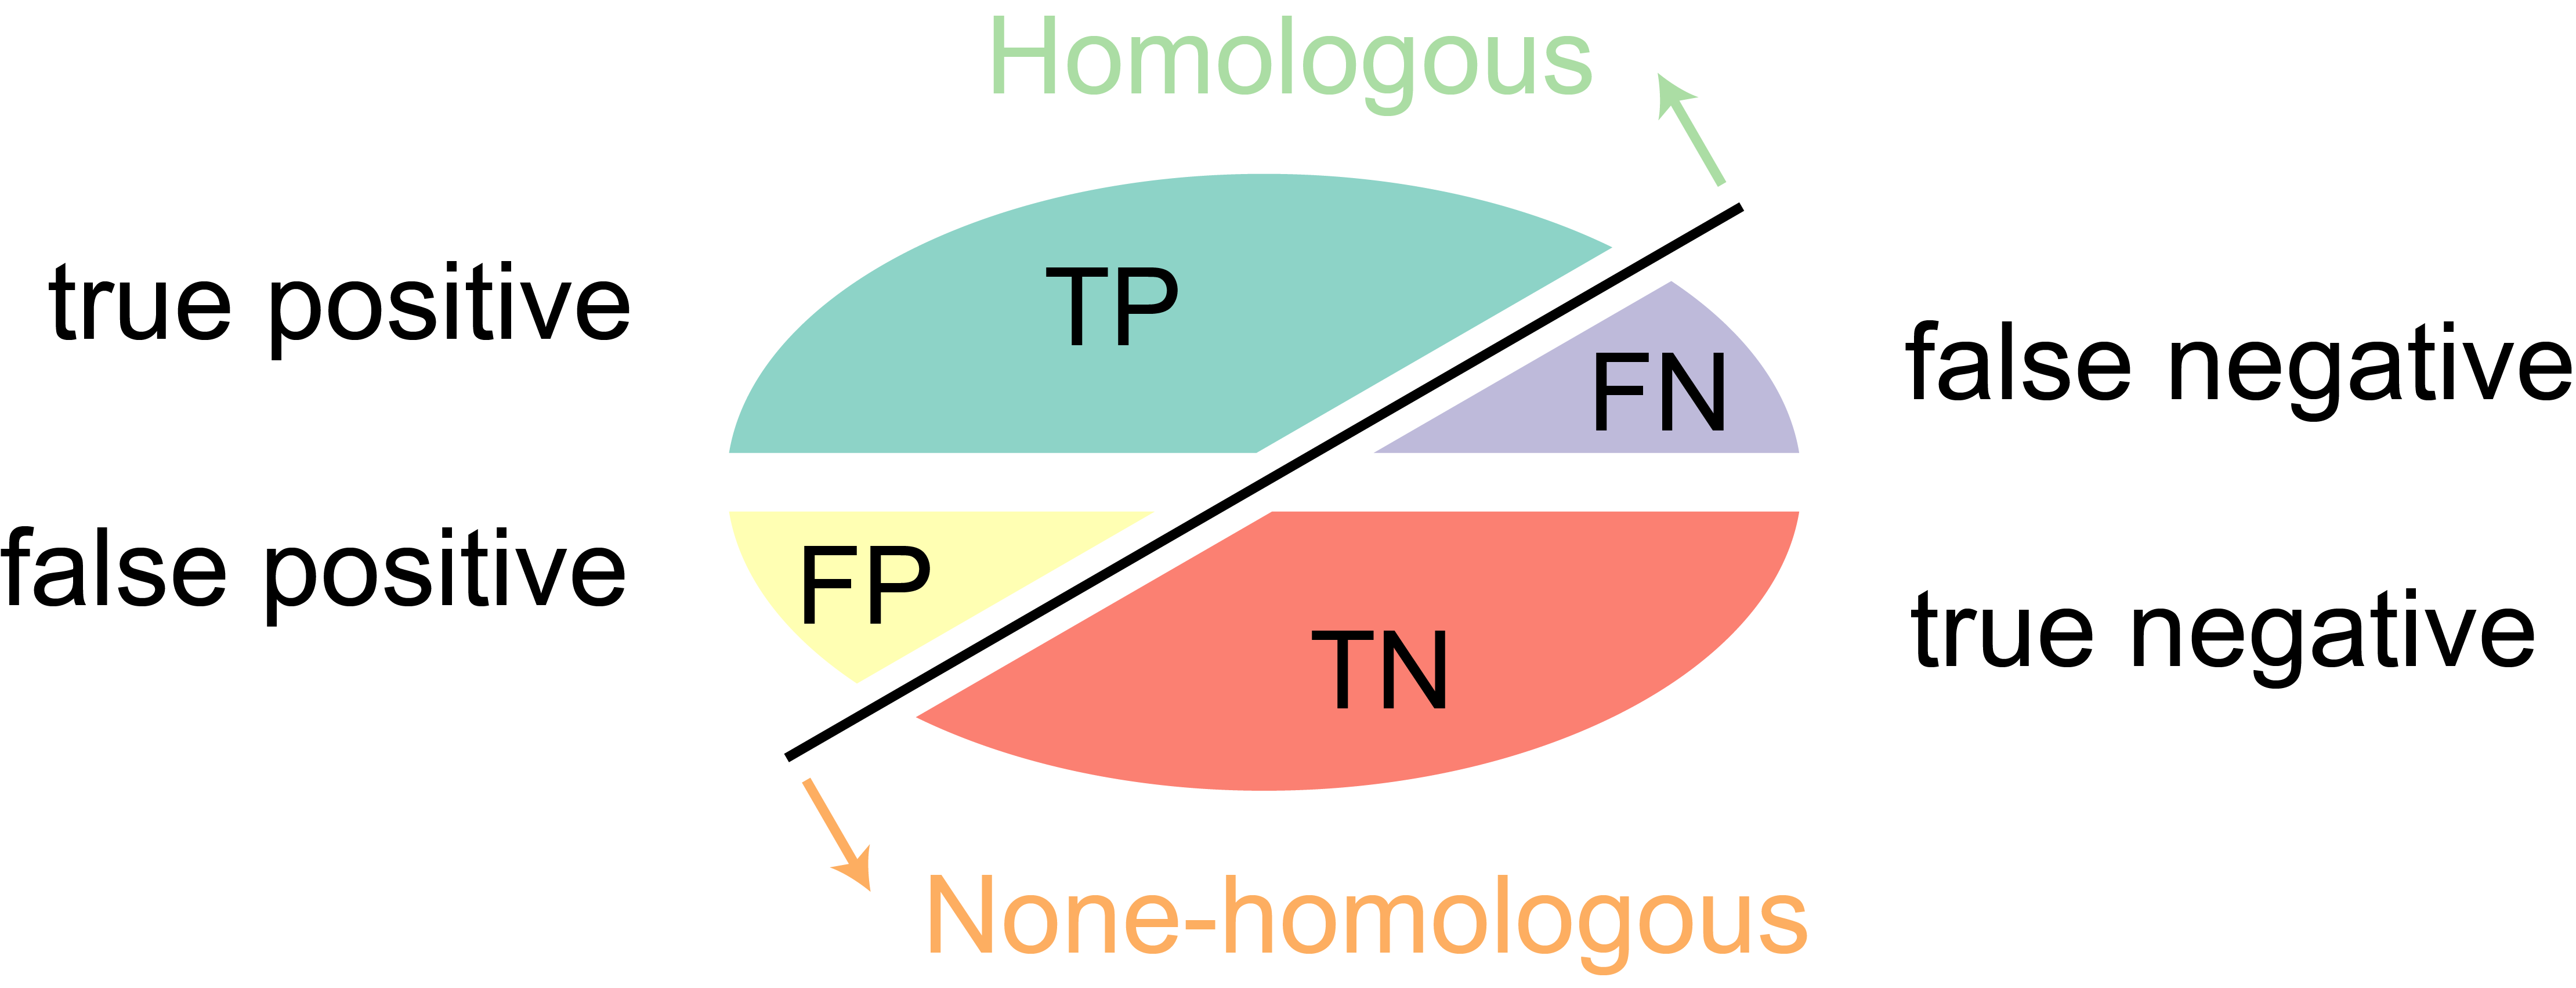
\includegraphics[width=0.4 \textwidth]{fig07/four_outcomes.png}
  \caption{Four outcomes of model classification}
\end{figure}


%
% Example of model output
%
\subsubsection*{Example of model output}
A test dataset contains 10 positives and 10 negative. 

\begin{figure}[H]
  \centering
      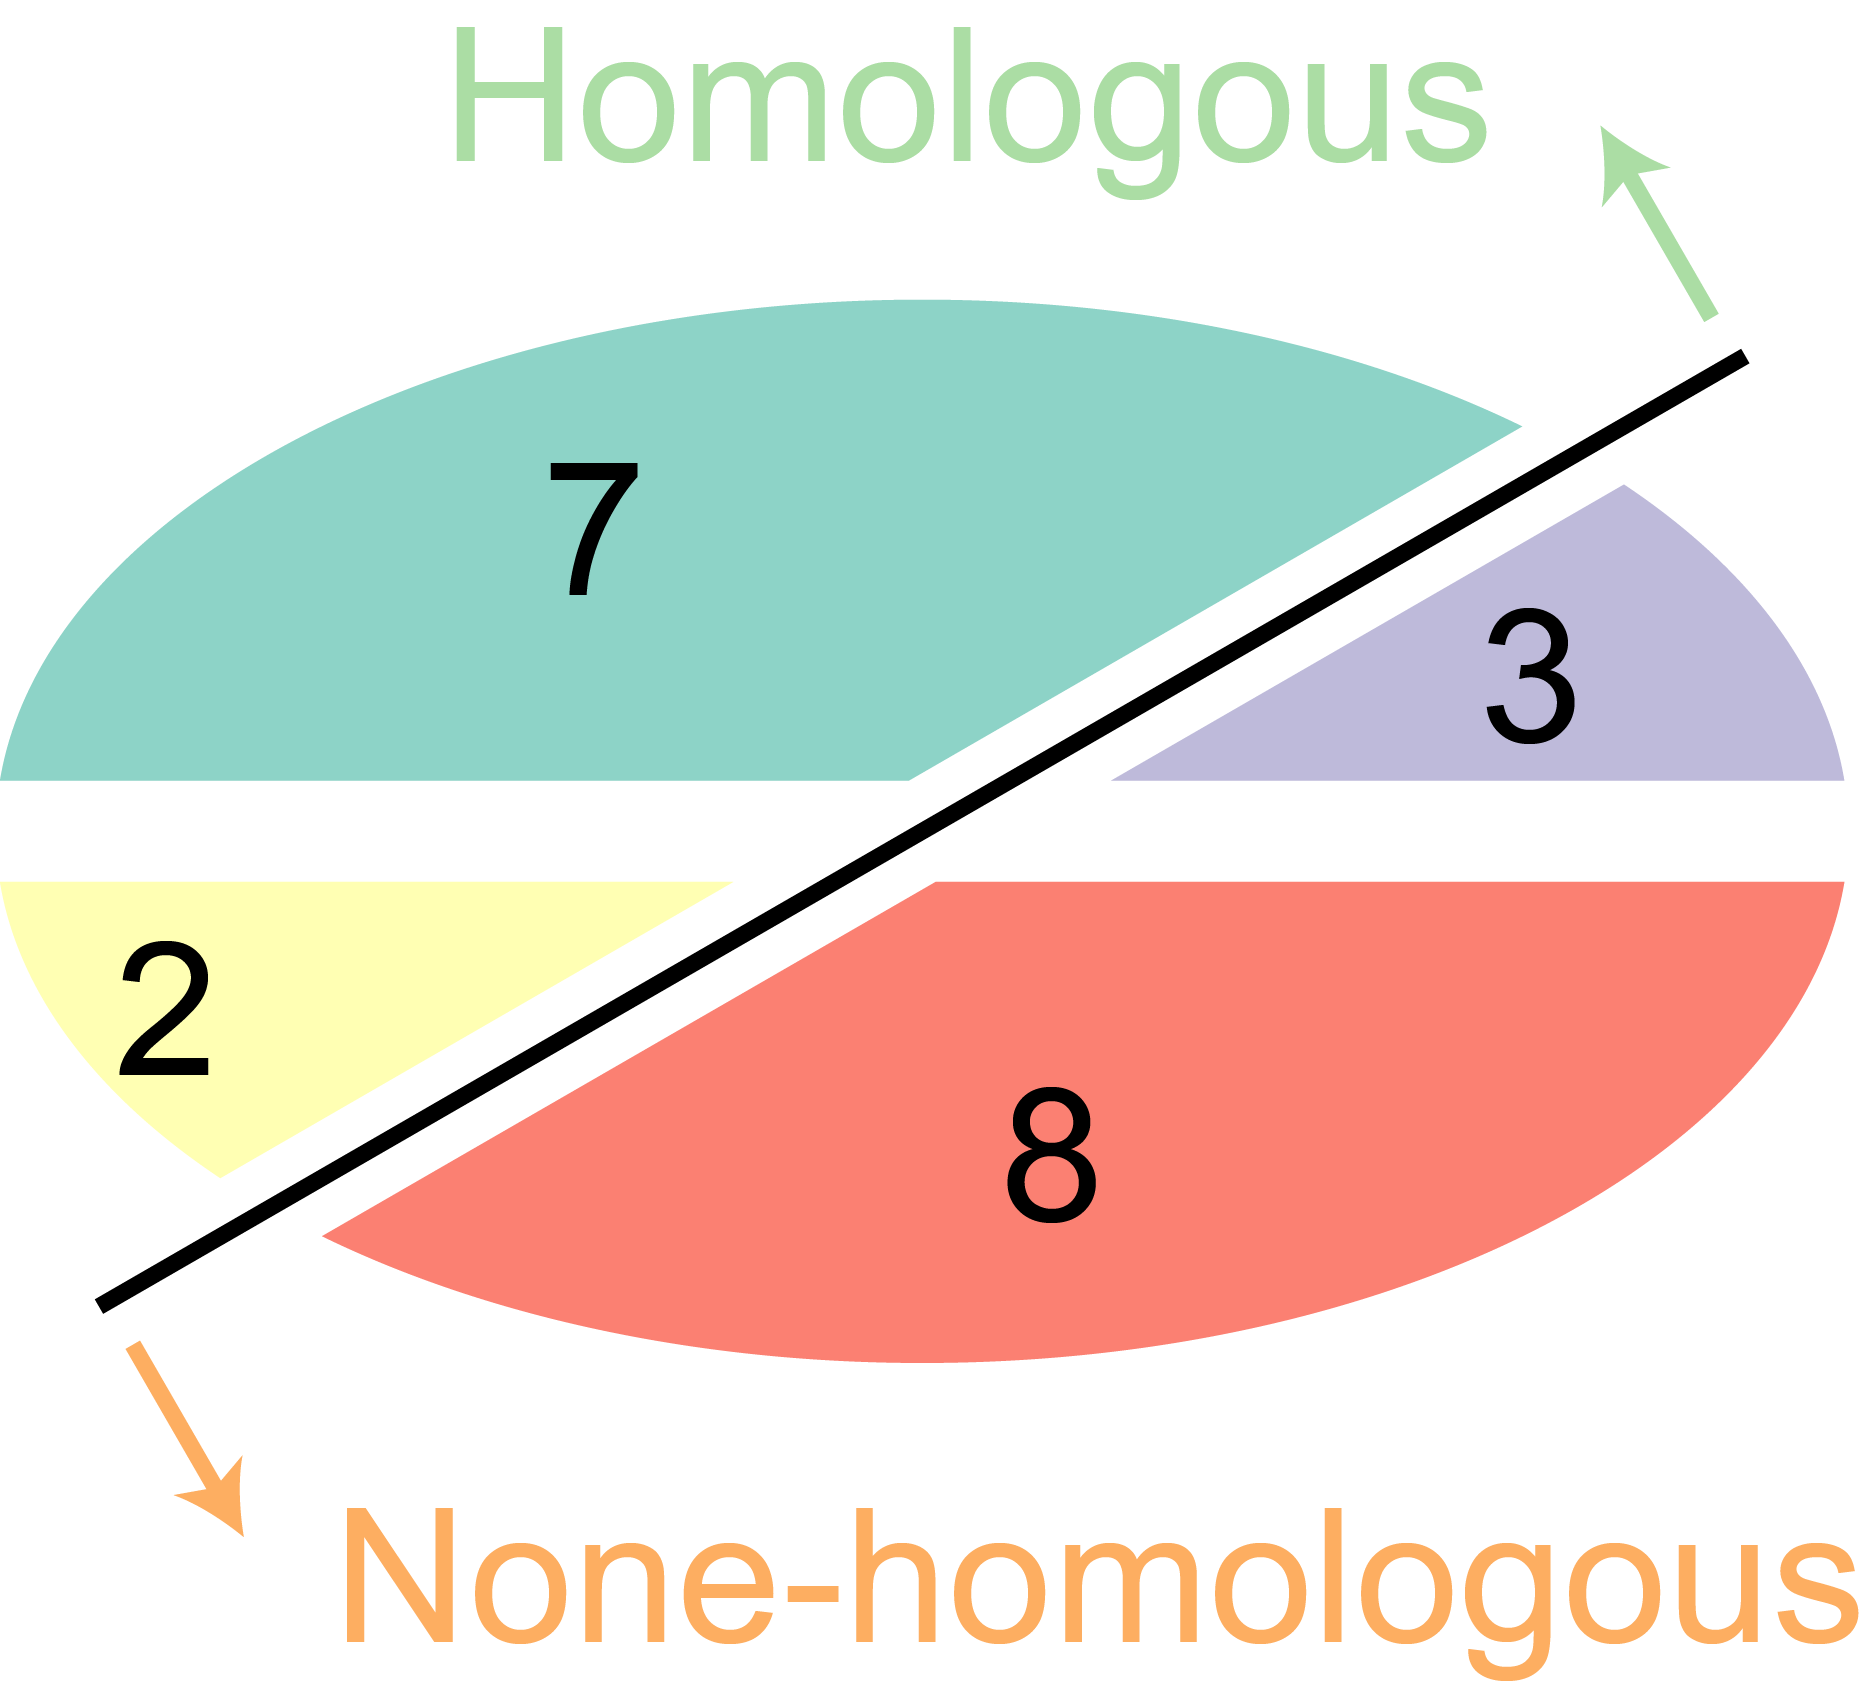
\includegraphics[width=0.2 \textwidth]{fig07/example_model_output.png}
  \caption{An example of the four outcomes}
\end{figure}

\begin{itemize}
\item 7 true positives
\item 8 true negatives
\item 2 false positives
\item 3 false negatives
\end{itemize}

%
% Confusion matrix
%
\subsubsection*{Confusion matrix}
The classification result can be formed into a matrix format.

\begin{table}[H]
\centering
\caption{Confusion matrix}
\begin{tabular}{ll|c|c|}
\cline{3-4}
                                                            &                & \multicolumn{2}{c|}{Test data}                                        \\ \cline{3-4} 
                                                            &                & \multicolumn{1}{l|}{Homologous} & \multicolumn{1}{l|}{Non-homologous} \\ \hline
\multicolumn{1}{|l|}{\multirow{2}{*}{Model classification}} & Homologous     & TP                              & FP                                  \\ \cline{2-4} 
\multicolumn{1}{|l|}{}                                      & Non-homologous & FN                              & TN                                  \\ \hline
\end{tabular}
\end{table}

%
% Example of confusion matrix
%
\subsubsection*{Example of confusion matrix}

\begin{table}[H]
\centering
\begin{tabular}{|l|l|}
\hline
7 TPs & 2 FPs \\ \hline
3 FNs & 8 TNs \\ \hline
\end{tabular}
\end{table}

\bigskip 

%\end{document}

\newpage
%\documentclass[12pt]{article}
%\usepackage[a4paper, margin=1in]{geometry} 
%\usepackage{graphicx} 
%\usepackage{hyperref}
%\usepackage{float}
%\usepackage{multicol}
%\usepackage{multirow}
%\usepackage[font=small, labelfont=bf]{caption}
%\usepackage{amssymb}
%\usepackage{amsmath}
%
%\begin{document}

%
% Basic evaluation measures 
%
\subsection{Basic evaluation measures}
Various measures can be derived from the confusion matrix.

%
% Accuracy
%
\subsubsection*{Accuracy}

$\dfrac{TP+TN}{TP+FP+TN+FN} = \dfrac{TP+TN}{P+N} $
\begin{figure}[H]
  \centering
      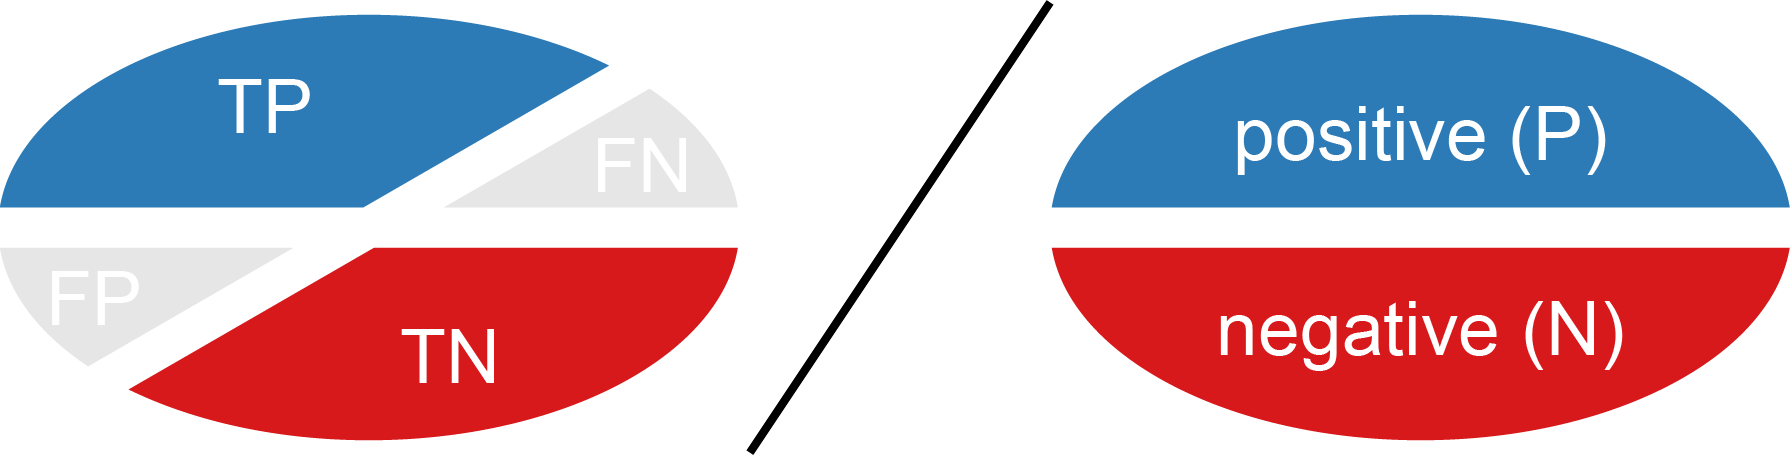
\includegraphics[width=0.4 \textwidth]{fig07/accuracy.png}
\end{figure}

%
% Error rate
%
\subsubsection*{Error rate}

$\dfrac{FP+FN}{TP+FP+TN+FN}= \dfrac{FP+FN}{P+N} $

\begin{figure}[H]
  \centering
      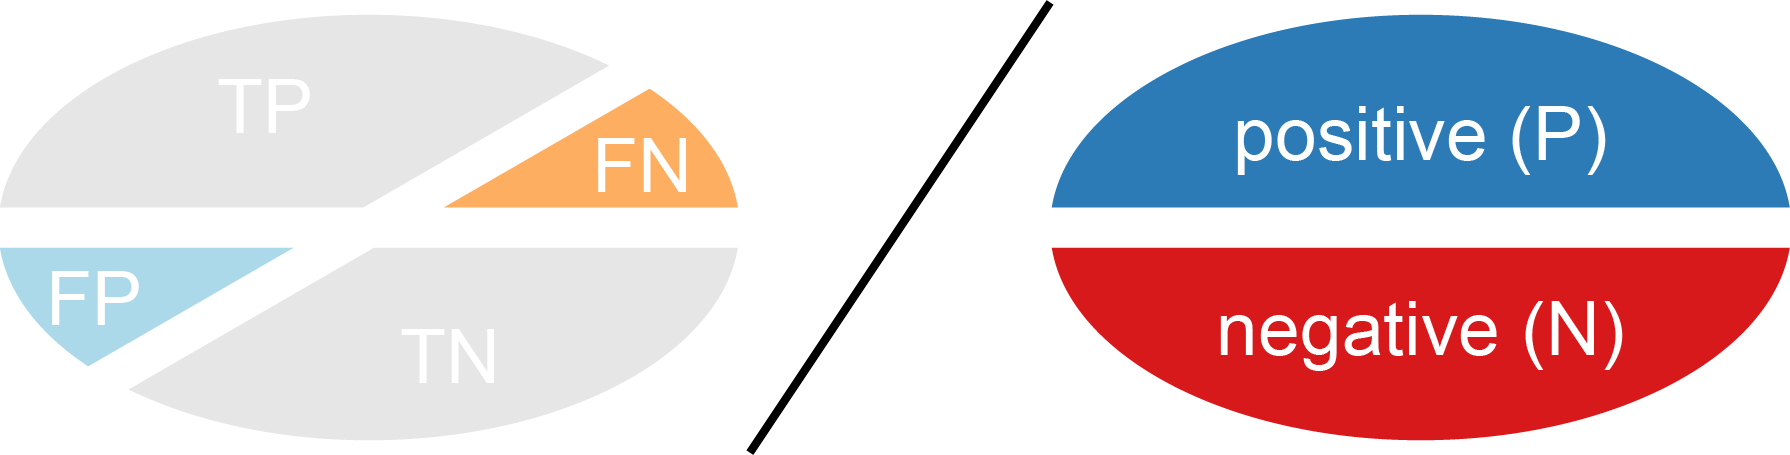
\includegraphics[width=0.4 \textwidth]{fig07/error-rate.png}
\end{figure}

%
% Sensitivity, True positive rate, Recall
%
\subsubsection*{Sensitivity, True positive rate, Recall}

$\dfrac{TP}{TP+FN}= \dfrac{TP}{P} $

\begin{figure}[H]
  \centering
      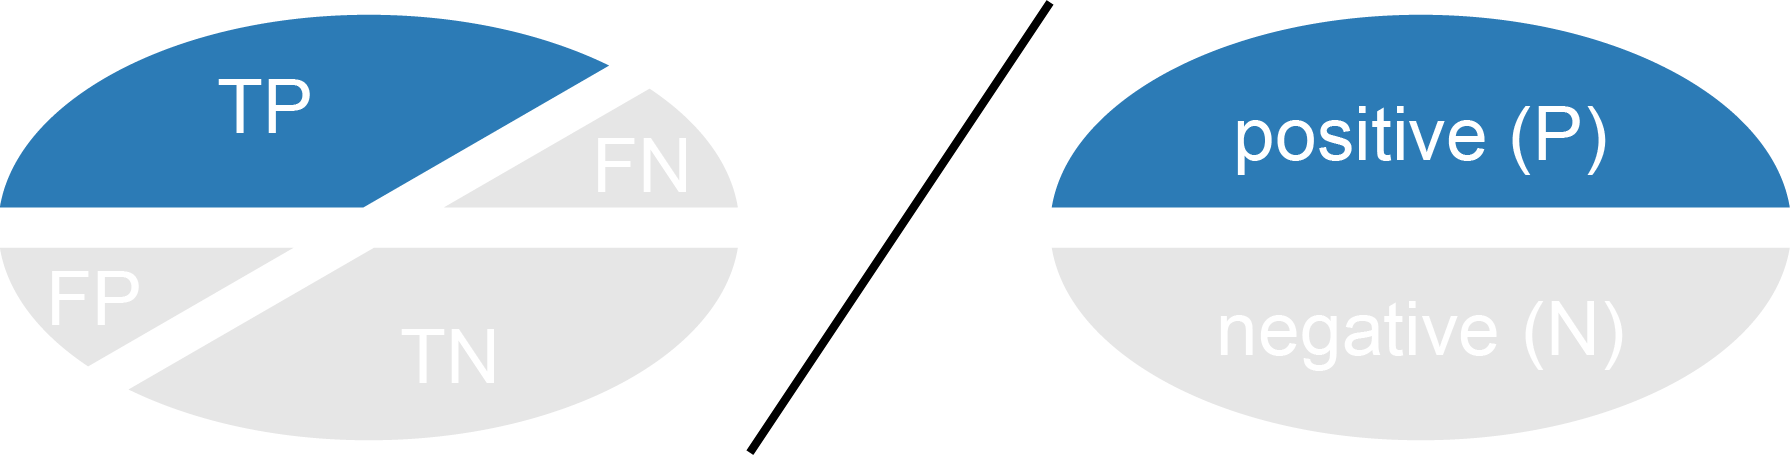
\includegraphics[width=0.4 \textwidth]{fig07/sensitivity.png}
\end{figure}

%
% Specificity, True negative rate
%
\subsubsection*{Specificity, True negative rate}

$\dfrac{TN}{FP+TN}= \dfrac{TN}{N} $

\begin{figure}[H]
  \centering
      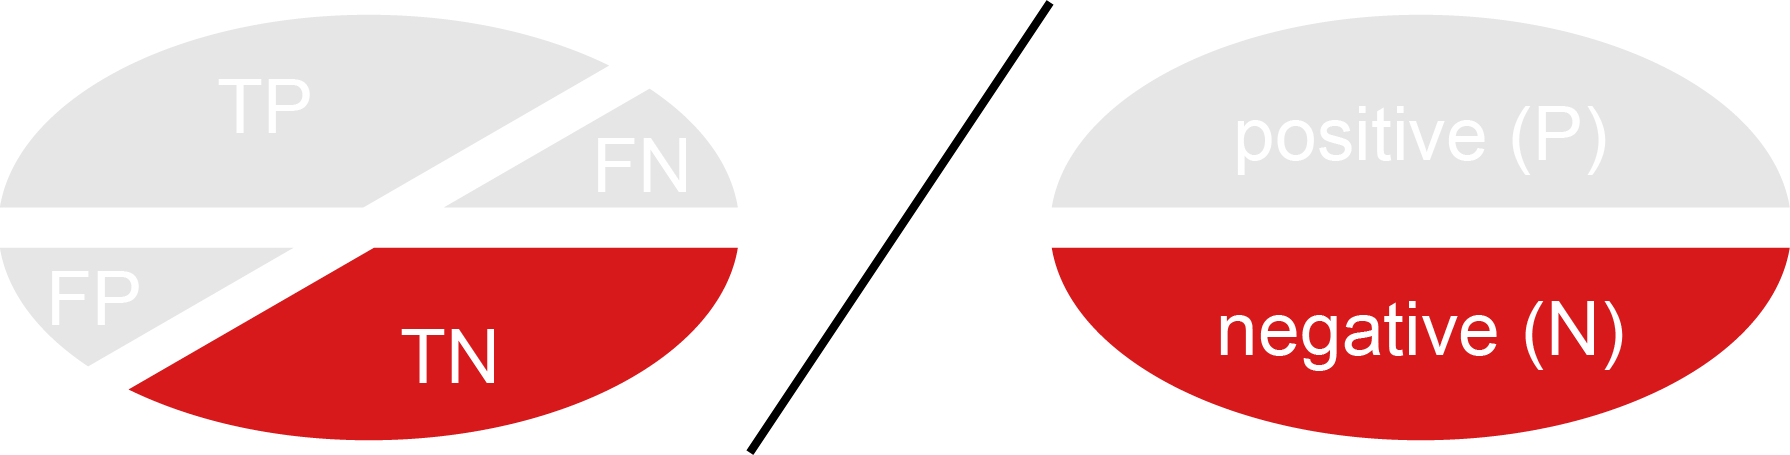
\includegraphics[width=0.4 \textwidth]{fig07/specificity.png}
\end{figure}

%
% Precision, Positive predictive value
%
\subsubsection*{Precision, Positive predictive value}

$\dfrac{TP}{TP+FP}$

\begin{figure}[H]
  \centering
      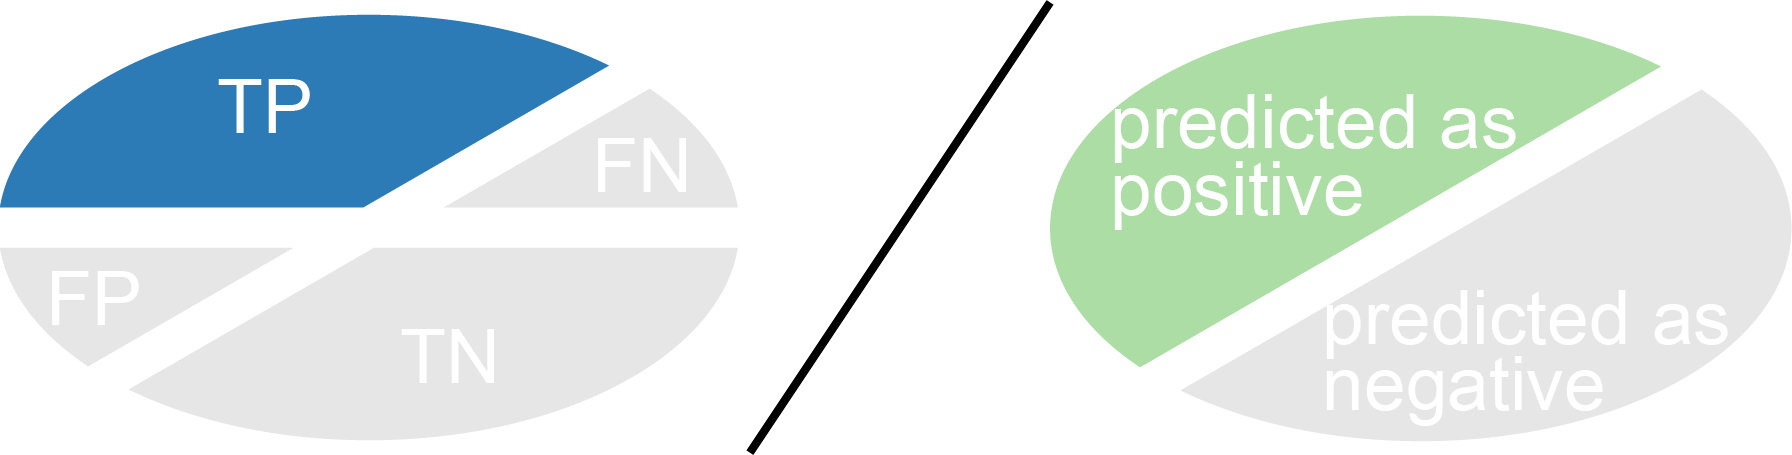
\includegraphics[width=0.4 \textwidth]{fig07/precision.png}
\end{figure}

\bigskip 

%\end{document}

%\documentclass[12pt]{article}
%\usepackage[a4paper, margin=1in]{geometry} 
%\usepackage{graphicx} 
%\usepackage{hyperref}
%\usepackage{float}
%\usepackage{multicol}
%\usepackage{multirow}
%\usepackage[font=small, labelfont=bf]{caption}
%\usepackage{amssymb}
%\usepackage{amsmath}
%
%\begin{document}

%
% Measures with multiple thresholds
%
\subsection{Measures with multiple thresholds}
The test data set needs to be sorted by scores, and then confusion matrices can be calculated for multiple threshold values.

%
% Example of making confusion matrices with multiple thresholds
%
\subsubsection*{Example of making confusion matrices with multiple thresholds}

\noindent
Test data set
\begin{table}[H]
\centering
\scriptsize
\begin{tabular}{|l|l|l|l|l|l|l|l|l|l|l|l|l|l|l|l|l|l|l|l|l|}
\hline
Label & N  & P & P  & N & N  & N & P  & P  & P  & N & P  & N & P  & P  & N  & N & P  & P  & N  & N \\ \hline
Score & 27 & 4 & 17 & 9 & 11 & 2 & 15 & 19 & 22 & 3 & 23 & 7 & 10 & 25 & 11 & 1 & 26 & 28 & 24 & 3 \\ \hline
\end{tabular}
\end{table}

\noindent
Sorted test data set
\begin{table}[H]
\centering
\scriptsize
\begin{tabular}{lllllllllllllllllllll}
\hline
\multicolumn{1}{|l|}{Label} & \multicolumn{1}{l|}{P}  & \multicolumn{1}{l|}{N}  & \multicolumn{1}{l|}{P}  & \multicolumn{1}{l|}{P}  & \multicolumn{1}{l|}{N}  & \multicolumn{1}{l|}{P}  & \multicolumn{1}{l|}{P}  & \multicolumn{1}{l|}{P}  & \multicolumn{1}{l|}{P}  & \multicolumn{1}{l|}{P}  & \multicolumn{1}{l|}{N}  & \multicolumn{1}{l|}{N}  & \multicolumn{1}{l|}{P}  & \multicolumn{1}{l|}{N} & \multicolumn{1}{l|}{N} & \multicolumn{1}{l|}{P} & \multicolumn{1}{l|}{N} & \multicolumn{1}{l|}{N} & \multicolumn{1}{l|}{N} & \multicolumn{1}{l|}{N} \\ \hline
\multicolumn{1}{|l|}{Score} & \multicolumn{1}{l|}{28} & \multicolumn{1}{l|}{27} & \multicolumn{1}{l|}{26} & \multicolumn{1}{l|}{25} & \multicolumn{1}{l|}{24} & \multicolumn{1}{l|}{23} & \multicolumn{1}{l|}{22} & \multicolumn{1}{l|}{19} & \multicolumn{1}{l|}{17} & \multicolumn{1}{l|}{15} & \multicolumn{1}{l|}{11} & \multicolumn{1}{l|}{11} & \multicolumn{1}{l|}{10} & \multicolumn{1}{l|}{9} & \multicolumn{1}{l|}{7} & \multicolumn{1}{l|}{4} & \multicolumn{1}{l|}{3} & \multicolumn{1}{l|}{3} & \multicolumn{1}{l|}{2} & \multicolumn{1}{l|}{1} \\ \hline
\multirow{2}{*}{Threshold}  &                         &                         & \multicolumn{2}{c}{$\uparrow$}                             &                         &                         &                         &                         & \multicolumn{2}{c}{$\uparrow$}                             &                         &                         &                         &                        &                        & \multicolumn{2}{c}{$\uparrow$}                           &                        &                        &                        \\
                            &                         &                         & \multicolumn{2}{c}{1}                             &                         &                         &                         &                         & \multicolumn{2}{c}{2}                             &                         &                         &                         &                        &                        & \multicolumn{2}{c}{3}                           &                        &                        &                       
\end{tabular}
\end{table}

\noindent
1st threshold (score = 25.5)
\begin{table}[H]
\footnotesize
\begin{tabular}{|l|l|}
\hline
2 TPs & 1 FPs \\ \hline
8 FNs & 9 TNs \\ \hline
\end{tabular}
\end{table}

\noindent
2nd threshold (score = 16)
\begin{table}[H]
\footnotesize
\begin{tabular}{|l|l|}
\hline
7 TPs & 2 FPs \\ \hline
3 FNs & 8 TNs \\ \hline
\end{tabular}
\end{table}

\noindent
3rd threshold (score = 3.5)
\begin{table}[H]
\footnotesize
\begin{tabular}{|l|l|}
\hline
10 TPs & 6 FPs \\ \hline
0 FNs & 4 TNs \\ \hline
\end{tabular}
\end{table}

%
% ROC and precision-recall
%
\subsubsection*{ROC and precision-recall}
These measure are based on the confusion matrices of all possible threshold values.

\begin{itemize}
\item ROC (Receiver operating characteristic) plot
\item Precision-recall plot
\end{itemize}

\begin{figure}[H]
  \centering
      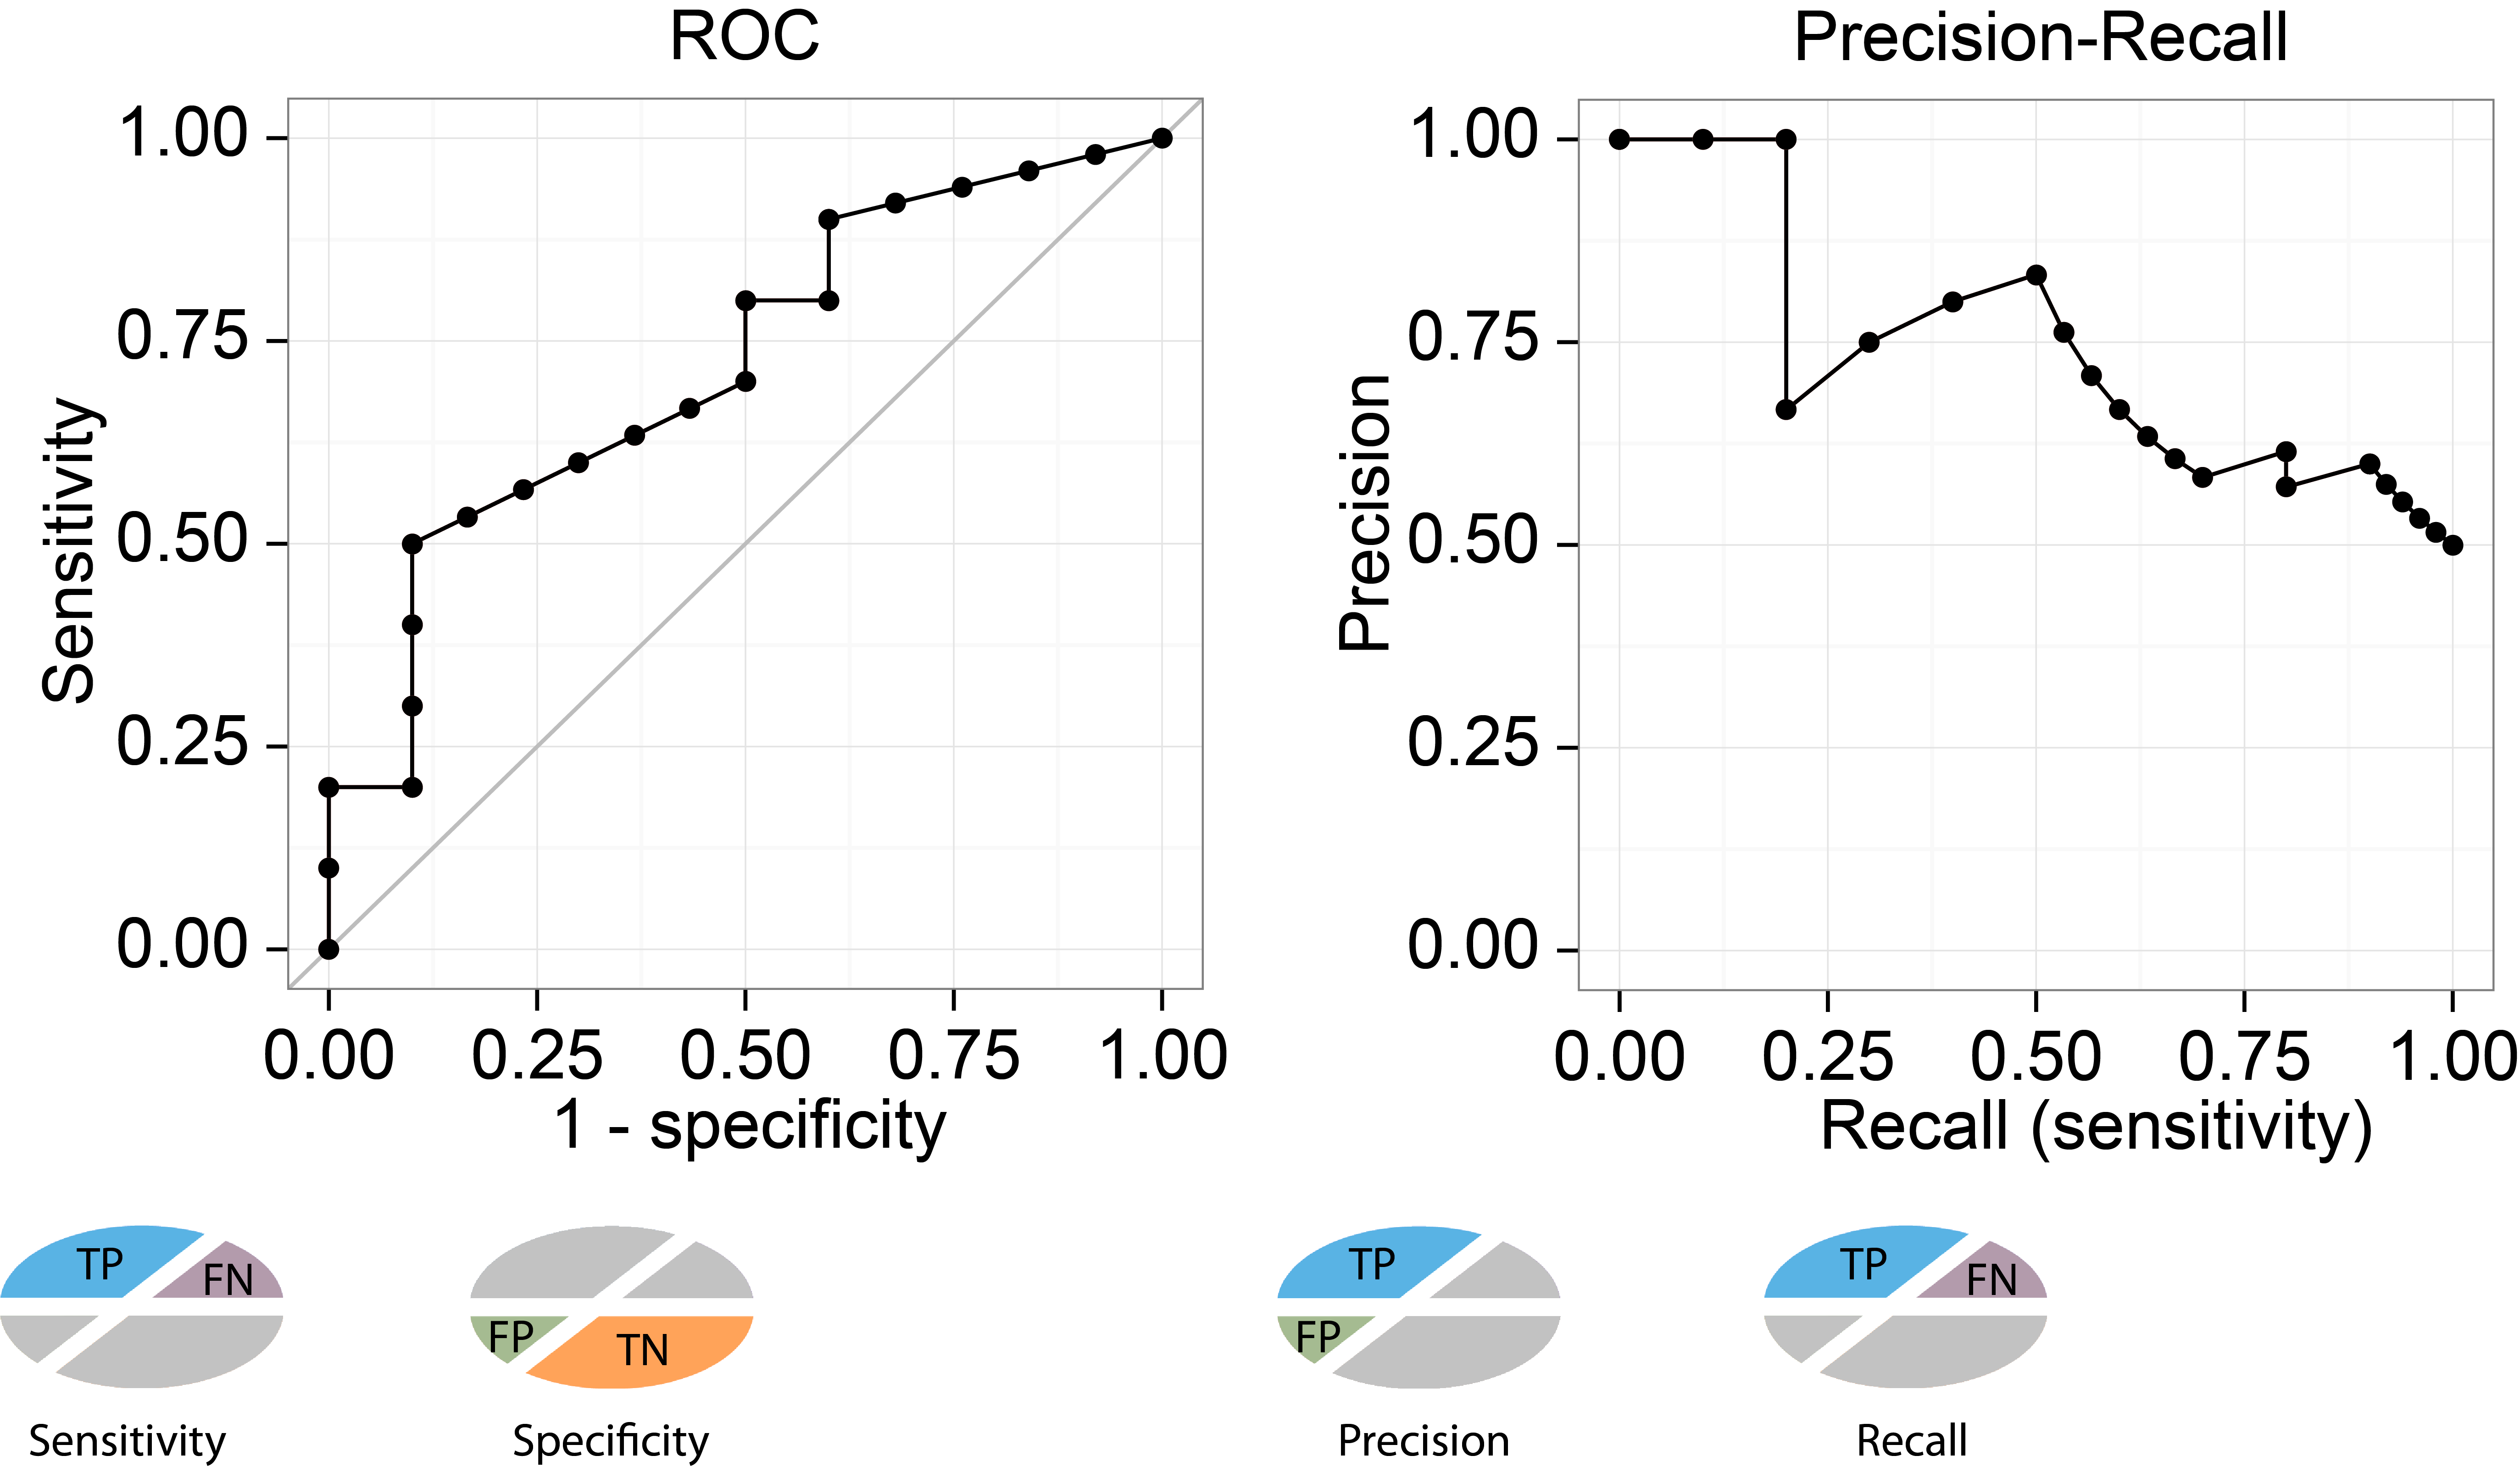
\includegraphics[width=0.6 \textwidth]{fig07/roc_precision-recall.png}
  \caption{ROC and precision-recall plots}
\end{figure}

%
% Exercise \thesection.1
%
\subsubsection*{Exercise \thesection.1}
Draw an ROC curve for the following specificity and sensitivity values.

\begin{table}[H]
\centering
\begin{tabular}{|l|l|l|l|}
\hline
Threshold & Specificity & 1 - Specificity & Sensitivity \\ \hline
10        & 1           & 0               & 0           \\ \hline
9         & 0.8         & 0.2             & 0.8         \\ \hline
8         & 0.6         & 0.4             & 0.8         \\ \hline
7         & 0.6         & 0.4             & 1           \\ \hline
6         & 0.4         & 0.6             & 1           \\ \hline
5         & 0.2         & 0.8             & 1           \\ \hline
4         & 0           & 1               & 1           \\ \hline
\end{tabular}
\end{table}

\begin{figure}[H]
  \centering
      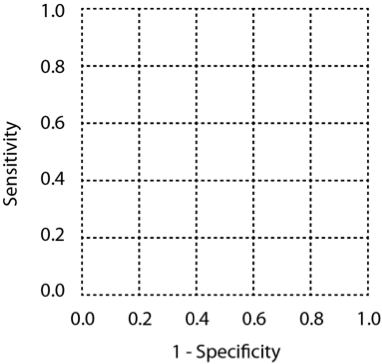
\includegraphics[width=0.4 \textwidth]{fig07/roc.png}
\end{figure}

\bigskip 

%\end{document}


\end{document}
